En los lotes de 50 cajas de los productos producidos por una determinada empresa (la población) producidos durante un determinado período con un total de 100 cajas se ha observado el número de piezas defectuosas (la variable estadística), presentado ésta un total de 11 modalidades, cuya distribución de frecuencias viene representado en la siguiente tabla:
\begin{center}
	\begin{table}[htbp]
		\begin{center}
			\begin{tabular}{|r|r|r|r|r|r|r|}
				\hline
				\multicolumn{1}{|l|}{$x_{i}$} & \multicolumn{1}{l|}{$n_{i}$} &
				\multicolumn{1}{l|}{$x_{i}n_{i}$} & \multicolumn{1}{l|}{$N_{i}$} & \multicolumn{1}{l|}{$n_{i}|x_{i} - \bar x|$} & \multicolumn{1}{l|}{$n_{i}|x_{i} - Me|$} & \multicolumn{1}{l|}{$n_{i}(x_{i} - \bar x)^2$} \\ \hline
				0 & 6 & 6 & 0 & 26,16 & 27,00 & 114,06 \\ \hline
				1 & 9 & 15 & 9 & 30,24 & 31,50 & 101,61 \\ \hline
				2 & 10 & 25 & 20 & 23,60 & 25,00 & 55,70 \\ \hline
				3 & 11 & 36 & 33 & 14,96 & 16,50 & 20,35 \\ \hline
				4 & 14 & 50 & 56 & 5,04 & 7,00 & 1,81 \\ \hline
				5 & 16 & 66 & 80 & 10,24 & 8,00 & 6,55 \\ \hline
				6 & 16 & 82 & 96 & 26,24 & 24,00 & 43,03 \\ \hline
				7 & 9 & 91 & 63 & 23,76 & 22,50 & 62,73 \\ \hline
				8 & 4 & 95 & 32 & 14,56 & 14,00 & 53,00 \\ \hline
				9 & 3 & 98 & 27 & 13,92 & 13,50 & 64,59 \\ \hline
				10 & 2 & 100 & 20 & 11,28 & 11,00 & 63,62 \\ \hline
			\end{tabular}
		\end{center}
	\end{table}
	
	
	
%\multicolumn{1}{|l|}{$x_{i}$} & \multicolumn{1}{l|}{$n_{i}$} & \multicolumn{1}{l|}{$N_{i}$} & \multicolumn{1}{l|}{$x_{i}n_{i}$} & \multicolumn{1}{l|}{$x_{i} - \bar x$} & \multicolumn{1}{l|}{$|x_{i} - \bar x|$} & \multicolumn{1}{l|}{$n_{i}|x_{i} - \bar x|$} & \multicolumn{1}{l|}{$|x_{i} - Me|$} & \multicolumn{1}{l|}{$n_{i}|x_{i} - Me|$} & \multicolumn{1}{l|}{$(x_{i} - \bar x)^2$} & \multicolumn{1}{l|}{$n_{i}(x_{i} - \bar x)^2$} \\	
	
\end{center}
a) La variable estadística observada es de carácter discreta, presentando un total de 11 modalidades: 0, 1, 2, 3, 4, 5, 6, 7, 8, 9 y 10. En este caso, la media más significativa es la aritmética, cuya expresión viene determinado por:

\begin{center}
	$\bar{x} = \frac{1}{n} \sum_{i=1}^{n}x_{i} n_{i}$ 
\end{center}

De la tabla podemos obtener que $\bar{x} = 4,36$ piezas. \\

b) La medida estadística que proporciona información sobre el número de piezas defectuosas que más habitualmente se puede esperar de una caja es la moda. Se define como $Mo = max(x_{i})$, con $i=1,2,3,...,n$. En este caso, se presentan dos modalidades que presentan la misma frecuencia absoluta. Por tanto, podemos afirmar que hay dos valores de moda en esta distribución, siendo más frecuente encontrar un total de 5 y 6 piezas defectuosas por lote examinado. \\

% Revisar concepto de mediana.
c) La mediana se define como un valor que divide a una determinada población en dos subgrupos con el mismo número de individuos: una de ellas cuyos individuos pertenecen a una modalidad cuya frecuencia absoluta es inferior a la mediana y otra con frecuencias absolutas superiores.

Para determinar la mediana en esta distribución de frecuencias, representamos la curva de distribución de la variable estadística: 

\begin{center}
	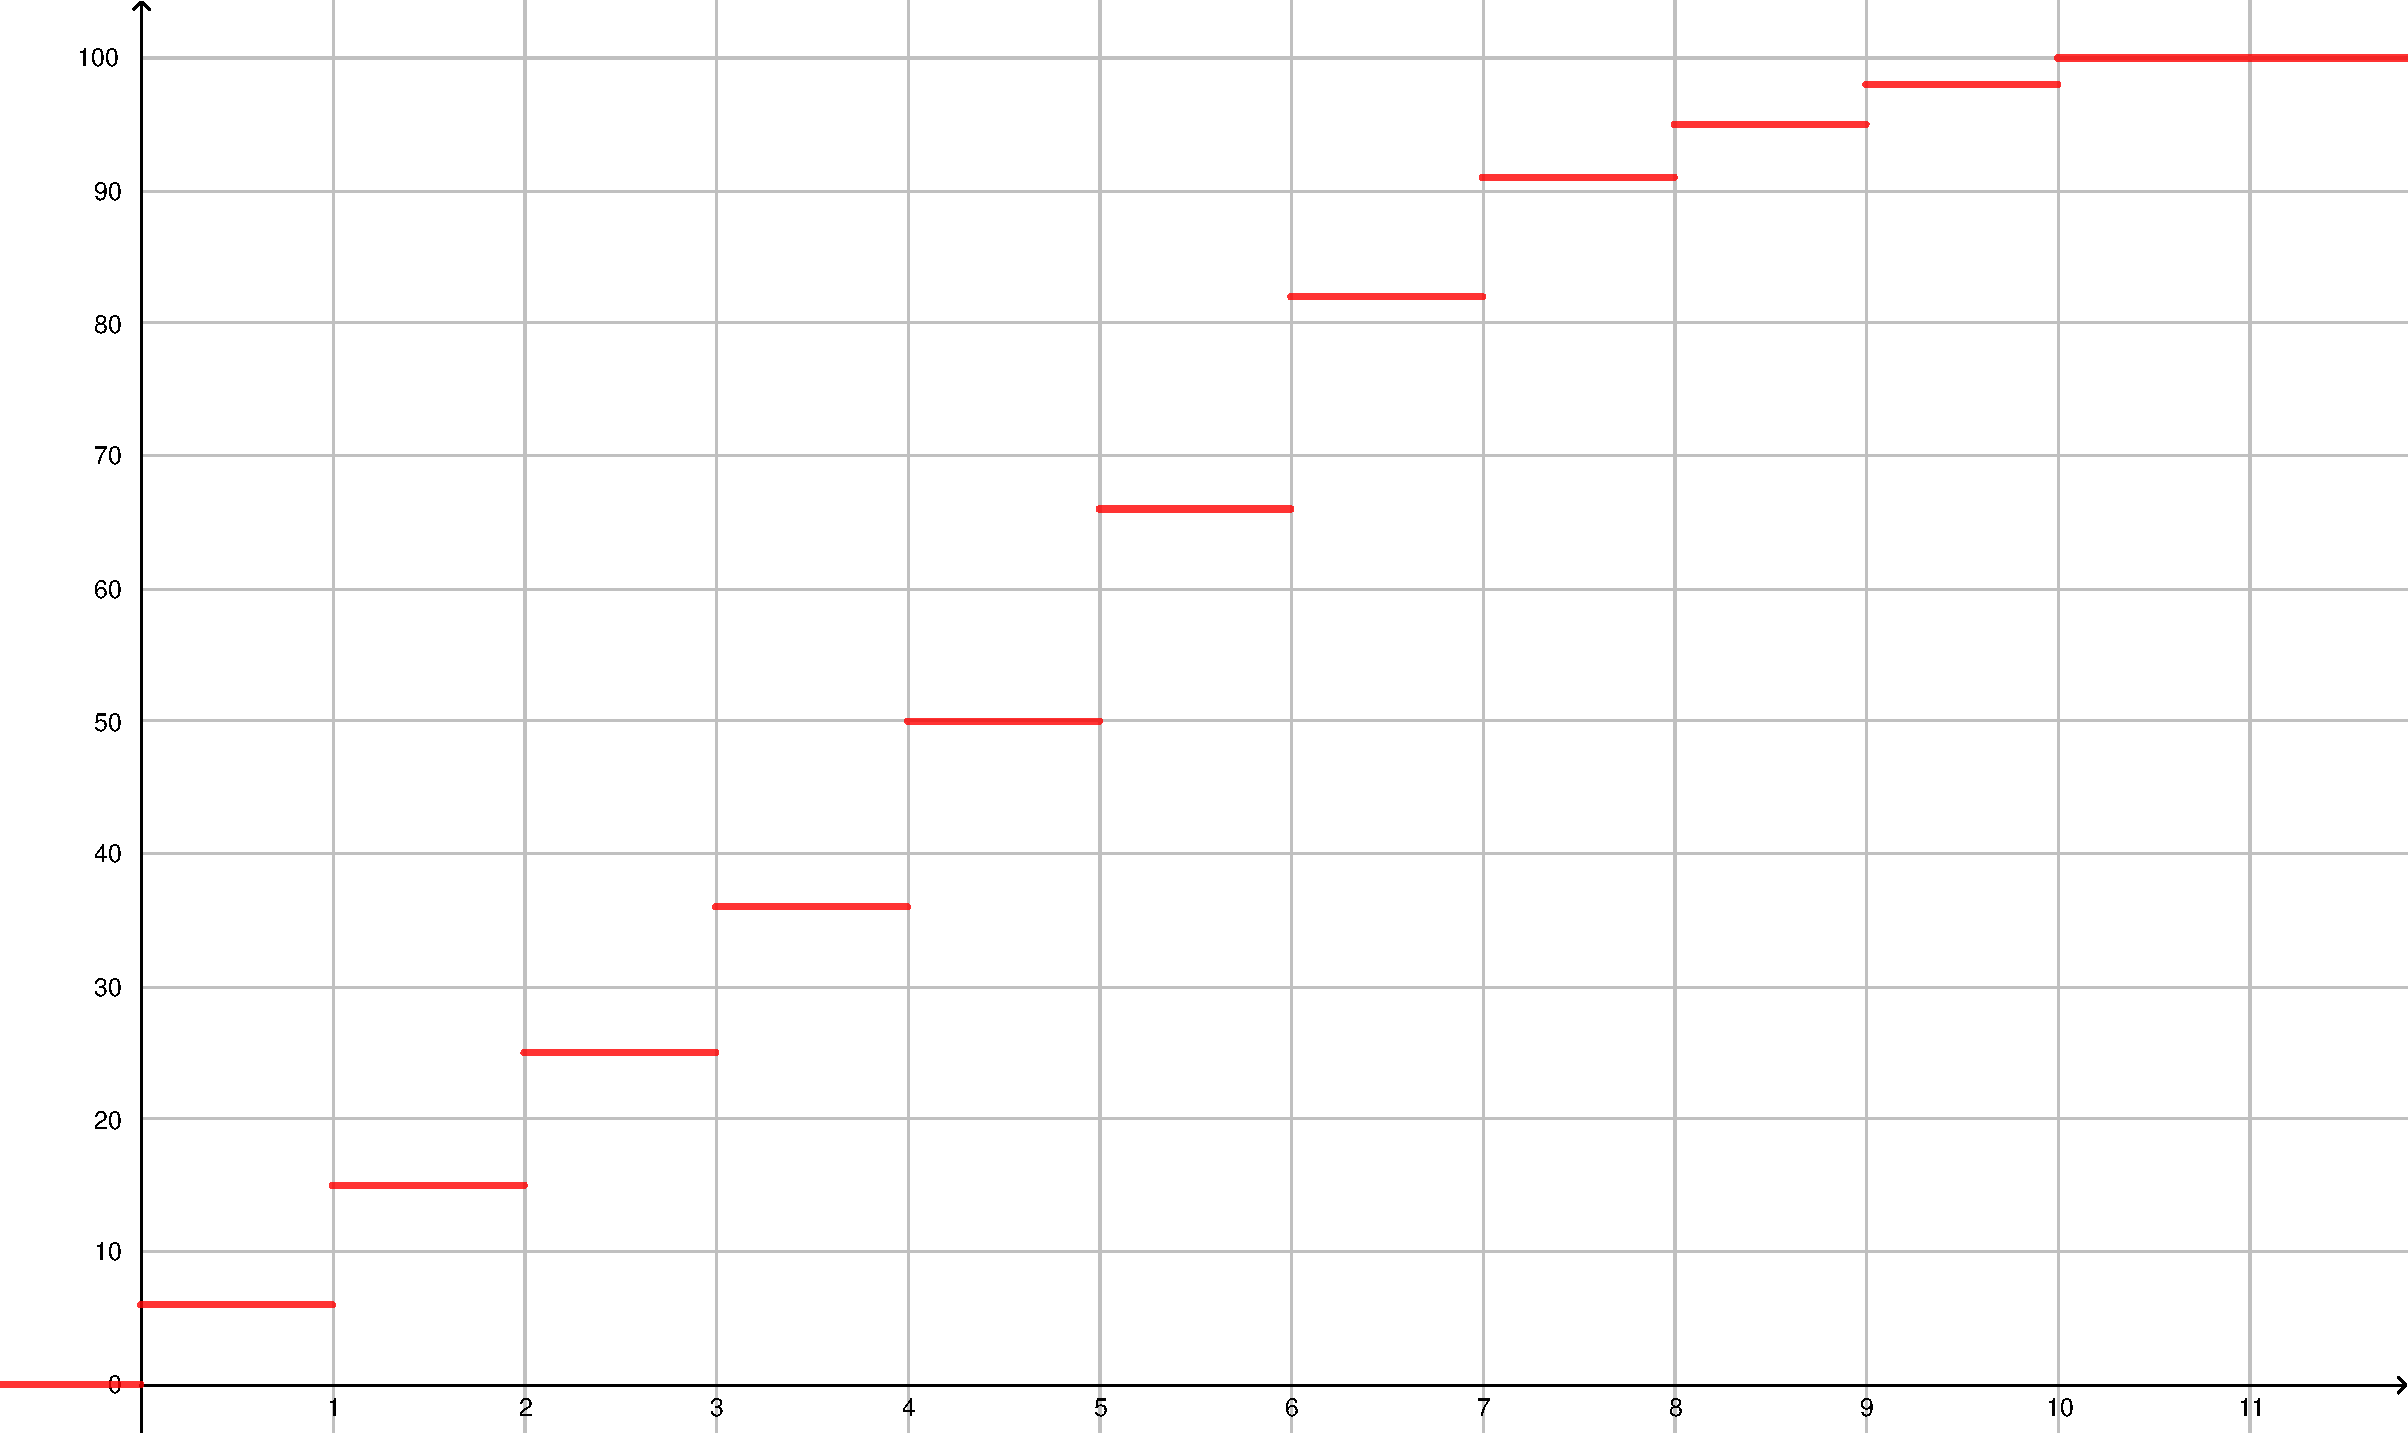
\includegraphics[scale=.35]{ejercicio-4-grafica.pdf}
\end{center}

Observamos que $\frac{n}{2} = 50$, coincidiendo justamente con el valor $F(x_{5}) = n/2$. Conviene pues tomar la media aritmética entre $x_{5}$ y $x_{6}$, de donde $Me = 4,5$ piezas defectuosas.

d) El cuartil es una medida que permite caracterizar el porcentaje de individuos de la población cuya variable estadística observada es inferior al $25\%, 50\%, 75\%$ de toda la población, respectivamente. Su cálculo es análogo al de la media (únicamente hay que sustituir $\frac{n}{2}$ por las fracciones correspondientes). De esta forma, deducimos las siguientes medidas:

$Q_{1} = 2,5$ piezas. Representa que un $25\%$ de los lotes analizados poseen una cantidad de productos defectuosos inferiores o iguales a 2,5 piezas.

$Q_{2} = 4,5$ piezas. Representa que un $50\%$ de los lotes analizados poseen una cantidad de productos defectuosos inferiores o iguales a 4,5 piezas.

$Q_{3} = 6$ piezas. Representa que un $75\%$ de los lotes analizados poseen una cantidad de productos defectuosos inferiores o iguales a 6 piezas.

e) El decil tiene un significado análogo a la de los cuartiles. Por tanto, el decil es una medida que permite caracterizar el porcentaje de individuos de la población cuya variable estadística observada es inferior al $10\%, 20\%,..., 90\%$ de toda la población. Su cálculo es, nuevamente, análogo a los casos anteriores: 

$D_{3} = 3$ piezas. Representa que un $30\%$ de los lotes analizados poseen una cantidad de productos defectuosos inferiores o iguales a 3 piezas.
$D_{7} = 6$ piezas. Representa que un $70\%$ de los lotes analizados poseen una cantidad de productos defectuosos inferiores o iguales a 6 piezas. \\

f) Algunas medidas de dispersión que podemos tomar sobre la variable estadística observada son las siguientes:

\begin{itemize}
	
	\item Recorrido. Es la magnitud que determina la anchura total de la muestra tomada (esto es, toma la diferencia entre el valor más alto tomado de la variable y el menor valor observado). Su ventaja es que tiene un significado concreto, pero su inconveniente es que varía mucho con fluctuaciones muestrales. En este caso, su valor es $R = 10$ piezas. Esto quiere decir que hay una variación de 10 productos defectuosos entre los datos de la muestra.
	
	\item Recorrido intercuartílico. Es la magnitud que indica la longitud del intervalo que contiene al $50\%$ central de los datos observados. Su virtud es que no varía mucho con fluctuaciones muestrales, pero su inconveniente es que no toma en consideración todos los datos de la población observada. En este caso, su valor es $R_{I} = 3,5$ piezas. Ello quiere decir que, del $50\%$ central de la muestra, hay, a lo sumo, una diferencia de 3,5 piezas defectuosas entre ellos.
	
	% Poner ventajas e inconvenientes.
	\item Desviación absoluta media respecto a la media. Indica cómo están los datos distribuidos en función del valor promedio (la media aritmética). Su valor es, en este caso, $D_{\bar x} = 2$ piezas.
	
	\item Desviación absoluta media respecto a la mediana. Significado y características análogos a la desviación absoluta media respecto a la media. Su valor es $D_{Me} = 2$ piezas, en este caso.
	
	\item Desviación típica. Es una medida que proporciona información sobre el margen óptimo de diferencia entre los valores medidos de la variable respecto de la media aritmética. Su principal ventaja es que proporciona una información que fluctúa poco, pero tiene el inconveniente de que requiere gran capacidad de cómputo para poder calcularse. Su valor es, en este caso, $\sigma_{x} = 2,42$ piezas.
	
	\item Recorrido relativo. Informa sobre el recorrido de la variable en función de su media aritmética. Su ventaja es que es fácil de calcular, pero tiene la desventaja de que varía mucho con las fluctuaciones estadísticas. En este caso, su valor es $R_{R} = 0,8$.
	
	\item Recorrido 
\end{itemize}

%$Var(X) = 5,85$ piezas al cuadrado.



$R_{SI} = 0,41$.
$C.V.(X) = 0,55$.
$V_{Me} = 0,44$.